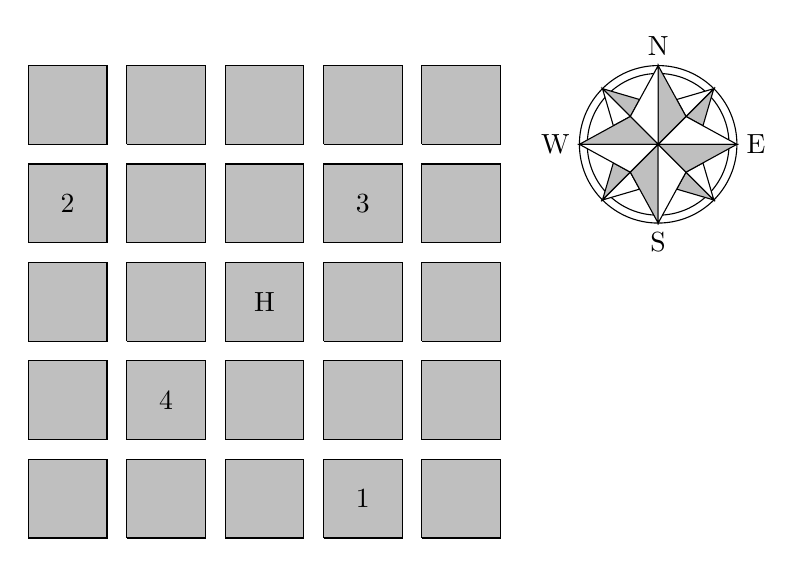
\begin{tikzpicture}
  %% Outer radius for the compass rose construction.
  \def\R{1}
  %% Inner radius for the compass rose construction.
  \def\r{.5}
  %% Width of "streets" in the map.
  \def\offset{0.25}
  %% Size of the "city block" in the map.
  \def\boxsize{1}
  %% One less than the number of "blocks" in the map
  \def\gridsize{4}
  
  %% Compute the center of the compass rose so it's in the top right of the map.
  \pgfmathsetmacro\CompassCenterX{{(\gridsize+3)*\boxsize + \gridsize*\offset}};
  \pgfmathsetmacro\CompassCenterY{{(\gridsize)*\boxsize + \gridsize*\offset}};
  
  %% Shift the compass rose so the center is where we want it.
  \def\xshift{\CompassCenterX}
  \def\yshift{\CompassCenterY}
  
  %% Draw the streets and blocks.
  \foreach \x in {0,...,\gridsize}
  \foreach \y in {0,...,\gridsize}
  \draw[fill=gray!50] (\x + \x*\offset, \y + \y*\offset)
  -- (\x + \x*\offset + \boxsize, \y + \y*\offset)
  -- (\x + \x*\offset + \boxsize , \y + \y*\offset +  \boxsize)
  -- (\x + \x*\offset , \y + \y*\offset + \boxsize)
  -- (\x + \x*\offset, \y + \y*\offset) ;

  %% Mark the locations.
  \node at (2*\boxsize + 2*\offset + \boxsize/2, 2*\boxsize + 2*\offset + \boxsize/2) {H};
  \node at (3*\boxsize + 3*\offset + \boxsize/2, 3*\boxsize + 3*\offset + \boxsize/2) {3};
  \node at (3*\boxsize + 3*\offset + \boxsize/2, \boxsize/2) {1};
  \node at (\boxsize/2, 3*\boxsize + 3*\offset + \boxsize/2) {2};
  \node at (\boxsize + \offset + \boxsize/2, \boxsize + \offset + \boxsize/2) {4};
  
  %% Draw the compass rose.
  \coordinate (O) at (\xshift, \yshift);
  \coordinate (N) at (\xshift,\R + \yshift);
  \coordinate (E) at (\R + \xshift, \yshift);
  \coordinate (S) at (\xshift,-\R + \yshift);
  \coordinate (W) at (-\R + \xshift, \yshift);
  
  %% The cirlces on the outside of the compass.
  \draw (\xshift,\yshift) circle (.9*\R);
  \draw (\xshift,\yshift) circle (\R);
  
  %% The points P1, ..., P4 are the inner points on the foreground star.
  \coordinate (P1) at ({\r*cos(45) + \xshift}, {\r*sin(45) + \yshift});
  \coordinate (P2) at ({\r*cos(135) + \xshift}, {\r*sin(135) + \yshift});
  \coordinate (P3) at ({\r*cos(225) + \xshift}, {\r*sin(225) + \yshift});
  \coordinate (P4) at ({\r*cos(315) + \xshift} , {\r*sin(315) + \yshift});
  
  
  %% The points Q1, ..., Q8 are the points where the two stars intersect.
  \coordinate (Q1) at ({\R*\r*sin(45)/(\r*cos(45)-\R)/(\r*sin(45)/(\r*cos(45)-\R) - tan(22.5)) + \xshift},{tan(22.5)*\R*\r*sin(45)/(\r*cos(45)-\R)/(\r*sin(45)/(\r*cos(45)-\R) - tan(22.5)) + \yshift});
  \coordinate (Q2) at ({\R/(tan(67.5) - (\r*sin(45)-\R)/(\r*cos(45))) + \xshift}, {\R/(tan(67.5) - (\r*sin(45)-\R)/(\r*cos(45)))*tan(67.5) + \yshift});
  \coordinate (Q3) at ({-\R/(tan(67.5) - (\r*sin(45)-\R)/(\r*cos(45))) + \xshift}, {\R/(tan(67.5) - (\r*sin(45)-\R)/(\r*cos(45)))*tan(67.5) + \yshift});
  \coordinate (Q4) at ({-\R*\r*sin(45)/(\r*cos(45)-\R)/(\r*sin(45)/(\r*cos(45)-\R) - tan(22.5)) + \xshift},{tan(22.5)*\R*\r*sin(45)/(\r*cos(45)-\R)/(\r*sin(45)/(\r*cos(45)-\R) - tan(22.5)) + \yshift});
  \coordinate (Q5) at ({-\R*\r*sin(45)/(\r*cos(45)-\R)/(\r*sin(45)/(\r*cos(45)-\R) - tan(22.5)) + \xshift},{-tan(22.5)*\R*\r*sin(45)/(\r*cos(45)-\R)/(\r*sin(45)/(\r*cos(45)-\R) - tan(22.5)) + \yshift});
  \coordinate (Q6) at ({-\R/(tan(67.5) - (\r*sin(45)-\R)/(\r*cos(45))) + \xshift}, {-\R/(tan(67.5) - (\r*sin(45)-\R)/(\r*cos(45)))*tan(67.5) + \yshift});
  \coordinate (Q7) at ({\R/(tan(67.5) - (\r*sin(45)-\R)/(\r*cos(45))) + \xshift}, {-\R/(tan(67.5) - (\r*sin(45)-\R)/(\r*cos(45)))*tan(67.5) + \yshift});
  \coordinate (Q8) at ({\R*\r*sin(45)/(\r*cos(45)-\R)/(\r*sin(45)/(\r*cos(45)-\R) - tan(22.5)) + \xshift},{-tan(22.5)*\R*\r*sin(45)/(\r*cos(45)-\R)/(\r*sin(45)/(\r*cos(45)-\R) - tan(22.5)) + \yshift});
  
  %% The points R1, ..., R4 are the points of the background star.
  \coordinate (R1) at ({\R*cos(45) + \xshift},{\R*sin(45) + \yshift});
  \coordinate (R2) at (({\R*cos(135) + \xshift}, {\R*sin(135) + \yshift});
  \coordinate (R3) at (({\R*cos(225) + \xshift}, {\R*sin(225) + \yshift});
  \coordinate (R4) at (({\R*cos(315) + \xshift}, {\R*sin(315) + \yshift});
  
  %% Compass headings
  \node [above] at (N) {N};
  \node [right] at (E) {E};
  \node [left] at (W) {W};
  \node [below] at (S) {S};
  
  %% Draw the background  star
  \draw [fill=gray!50] (Q1) -- (R1) -- (P1) -- (Q1);
  \draw [fill=white](Q2) -- (P1) -- (R1) -- (Q2);
  \draw [fill=gray!50] (Q3) -- (R2) -- (P2) -- (Q3);
  \draw [fill=white](Q4) -- (P2) -- (R2) -- (Q4);
  \draw [fill=gray!50] (Q5) -- (R3) -- (P3) -- (Q5);
  \draw [fill=white](Q6) -- (P3) -- (R3) -- (Q6);
  \draw [fill=gray!50] (Q7) -- (R4) -- (P4) -- (Q7);
  \draw [fill=white](Q8) -- (P4) -- (R4) -- (Q8);
  
  %% Draw the foreground star.
  \draw [fill=white] (O) -- (E) -- (P1) -- (O);
  \draw[fill=gray!50] (O) -- (P1) -- (N) -- (O);
  \draw [fill=white](O) -- (N) -- (P2) -- (O);
  \draw[fill=gray!50] (O) -- (P2) -- (W) -- (O);
  \draw [fill=white] (O) -- (W) -- (P3) -- (O);
  \draw [fill=gray!50] (O) -- (P3) -- (S) -- (O);
  \draw [fill=white] (O) -- (S) -- (P4) -- (O);
  \draw [fill=gray!50] (O) -- (P4) -- (E) -- (O);
\end{tikzpicture}
